\section{AWD-LSTM}
\begin{frame}[c]{Regularizing and Optimizing LSTM Language Models}
  \begin{itemize}
  	\setbeamertemplate{itemize items}[square]
  	\item Стратегии регуляризации, такие как dropout и batch normalization, не работают в случае рекуррентных нейронных сетей:
	\begin{itemize}
		\setbeamertemplate{itemize items}[circle]
		\item dropout нарушает способность RNN сохранять долгосрочные зависимости;
		\item batch normalization усложняет модель.
	\end{itemize}
	\setbeamertemplate{itemize items}[square]
	\item В статье предлагается набор эффективных стратегий регуляризации, которые могут быть использованы без изменения существующих реализаций LSTM.
  \end{itemize}
\let\thefootnote\footnote{\href{https://arxiv.org/abs/1708.02182}{\color[rgb]{0.5,0.5,0.5} [Merity et al., 2017]}}
\end{frame}

\begin{frame}[c]{Regularizing and Optimizing LSTM Language Models}
\begin{itemize} 
	\setbeamertemplate{itemize items}[square]
	\item Обычный dropout использует разные маски выбрасывания на разных временных шагах, без выбрасывания на повторяющихся слоях.
	\item Вариационный dropout использует одну и ту же маску выбрасывания на каждом временном шаге, включая повторяющиеся слои.
\end{itemize}
\begin{figure}
	\centering
	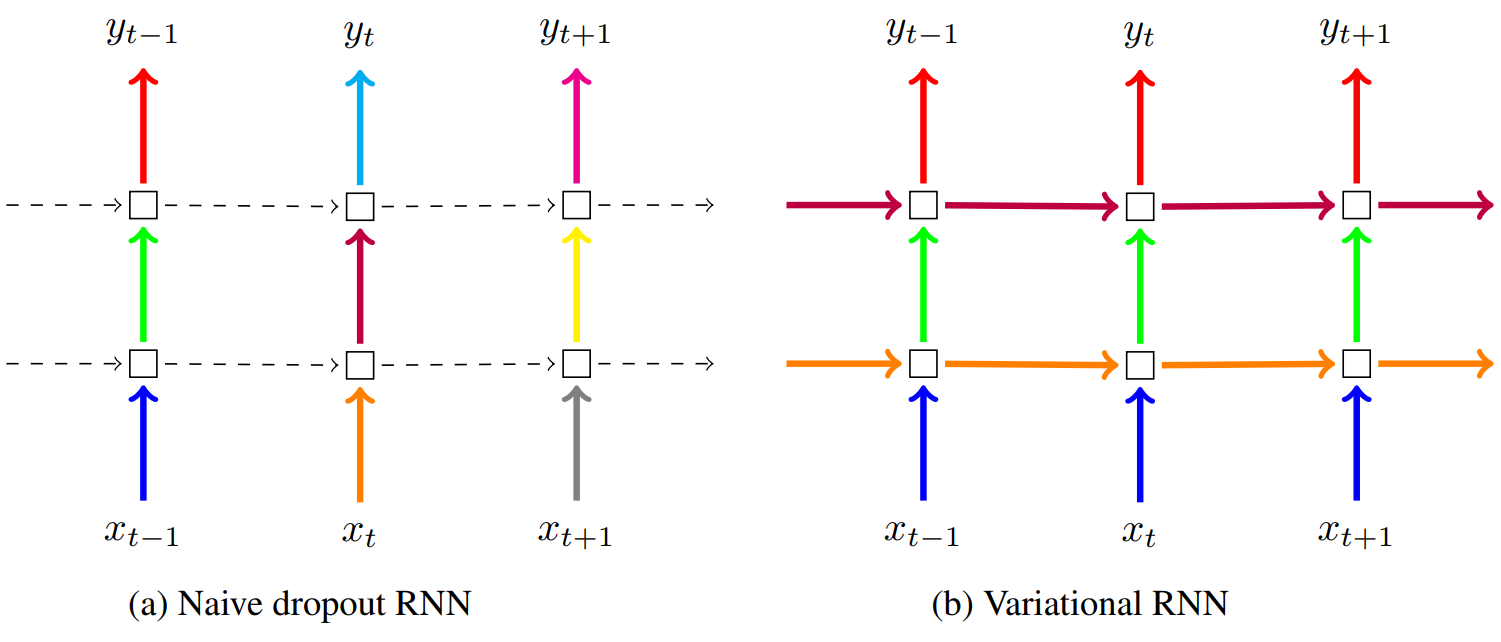
\includegraphics[width=0.9\textwidth]{figures/vardrop.png}
\end{figure}
\end{frame}


\begin{frame}[c]{Regularizing and Optimizing LSTM Language Models}
\begin{itemize}
	\setbeamertemplate{itemize items}[square]
	\item Dropout
\end{itemize}
\begin{figure}
	\centering
	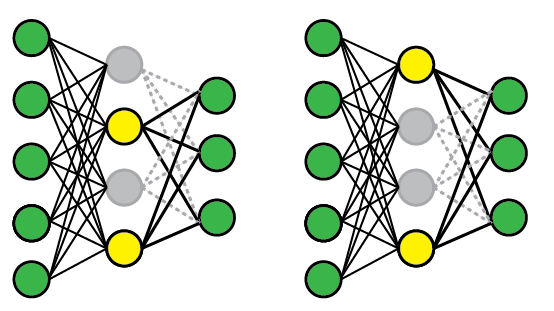
\includegraphics[width=0.8\textwidth]{figures/dropout.png}
\end{figure}

\end{frame}

\begin{frame}[c]{Regularizing and Optimizing LSTM Language Models}
\begin{itemize}
\setbeamertemplate{itemize items}[square]
\item DropConnect
\end{itemize}
\begin{figure}
\centering
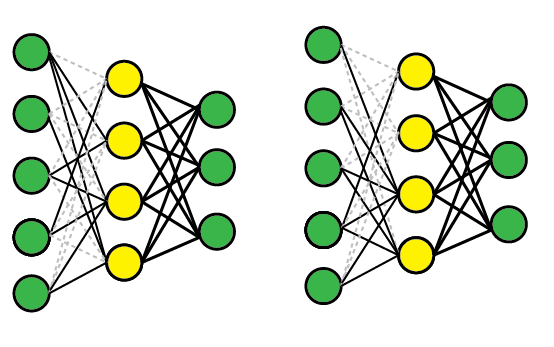
\includegraphics[width=0.8\textwidth]{figures/dropconnect.png}
\end{figure}

\end{frame}

\begin{frame}[c]{Regularizing and Optimizing LSTM Language Models}
  \begin{itemize}
	\setbeamertemplate{itemize items}[square]
	\item LSTM:
	\begin{itemize}
		\setbeamertemplate{itemize items}[circle]
		\item $i_t = \sigma\left(W^ix_t + U^ih_{t-1}\right)$
		\item $f_t = \sigma\left(W^fx_t + U^fh_{t-1}\right)$
		\item $o_t = \sigma\left(W^ox_t + U^oh_{t-1}\right)$
		\item $\overline{c}_t = \tanh\left(W^cx_t + U^ch_{t-1}\right)$	
		\item $c_t = i_t \circ \overline{c}_t + f_t \circ c_{t-1}$
		\item $h_t = o_t \circ \tanh\left(c_t\right)$
	\end{itemize}
	\setbeamertemplate{itemize items}[square]
	\item Вариационный DropConnect (WeightDrop) для весов: $\left[U^i, U^f, U^o, U^c\right].$ 
	\item Вариационный DropOut для весов: $\left[W^i, W^f, W^o, W^c\right].$ 
	\item Embedding DropOut: эквивалентно удалению слов из словаря. 
	\item Последовательности переменной длины.
	\item Weight tying: общие веса для embedding и softmax слоев.
	\item Activation Regularization (AR): $\alpha L_2(m \circ h_t)$.
	\item Temporal Activation Regularization (TAR): $\beta L_2(h_t - h_{t-1})$.
\end{itemize}
\end{frame}

\begin{frame}[c]{Regularizing and Optimizing LSTM Language Models}
\begin{itemize}
	\setbeamertemplate{itemize items}[square]
	\item Результаты (perplexity) на данных Penn Treebank:
	\begin{figure}
		\centering
		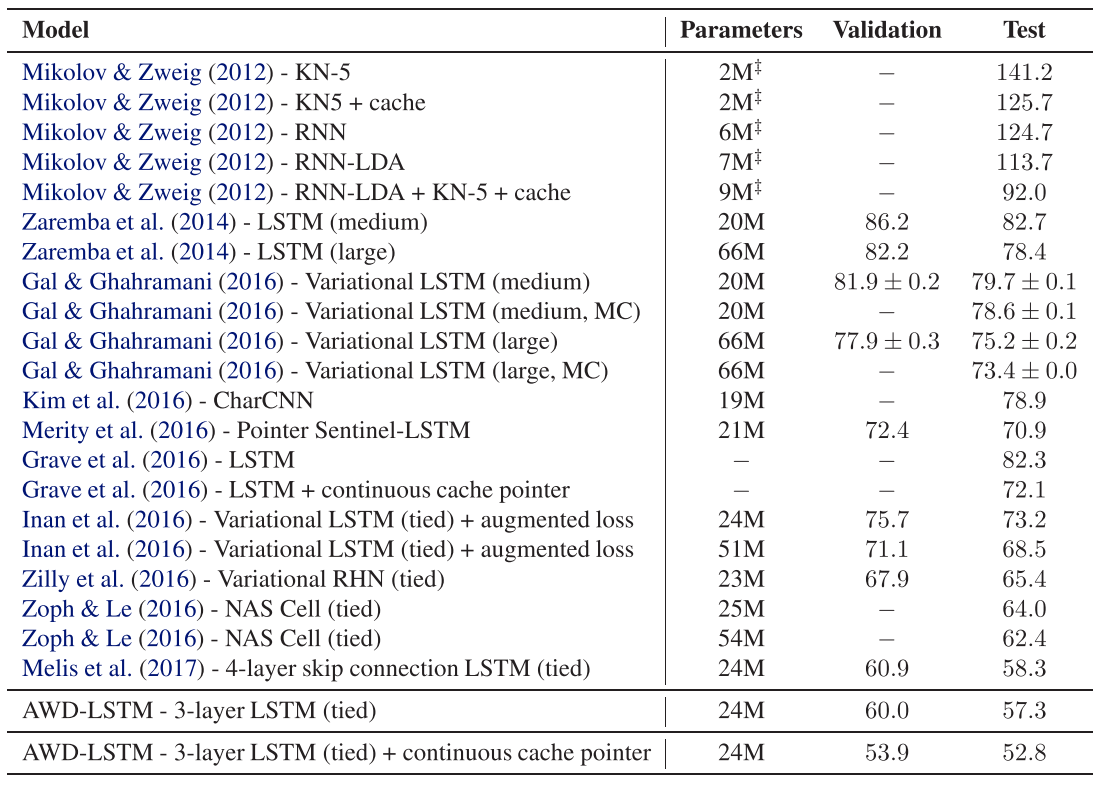
\includegraphics[width=0.8\textwidth]{figures/awdres.png}
	\end{figure}
\end{itemize}
\end{frame}

\begin{frame}[c]{Regularizing and Optimizing LSTM Language Models}
\begin{itemize}
	\setbeamertemplate{itemize items}[square]
	\item Результаты (perplexity) на данных WikiText-2:
	\begin{figure}
		\centering
		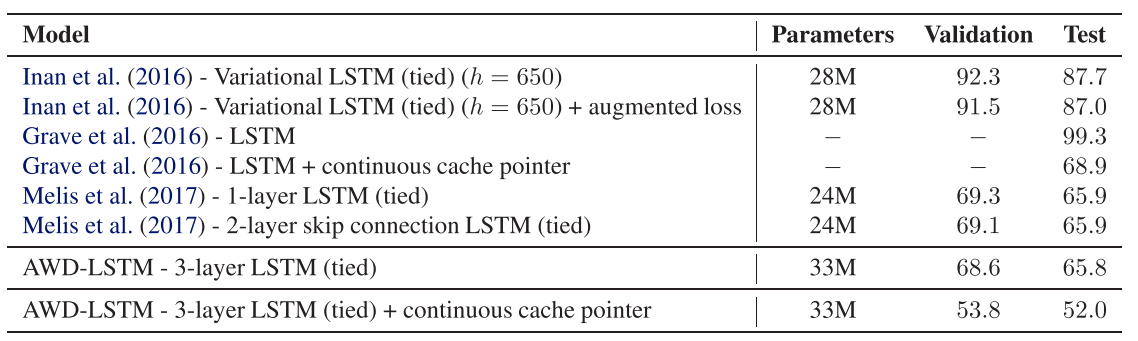
\includegraphics[width=0.9\textwidth]{figures/awdres1.png}
	\end{figure}
\end{itemize}
\end{frame}

\begin{frame}[c]{Regularizing and Optimizing LSTM Language Models}
\begin{itemize}
	\setbeamertemplate{itemize items}[square]
	\item Результаты при удалении каждой формы регуляризации:
	\begin{figure}
		\centering
		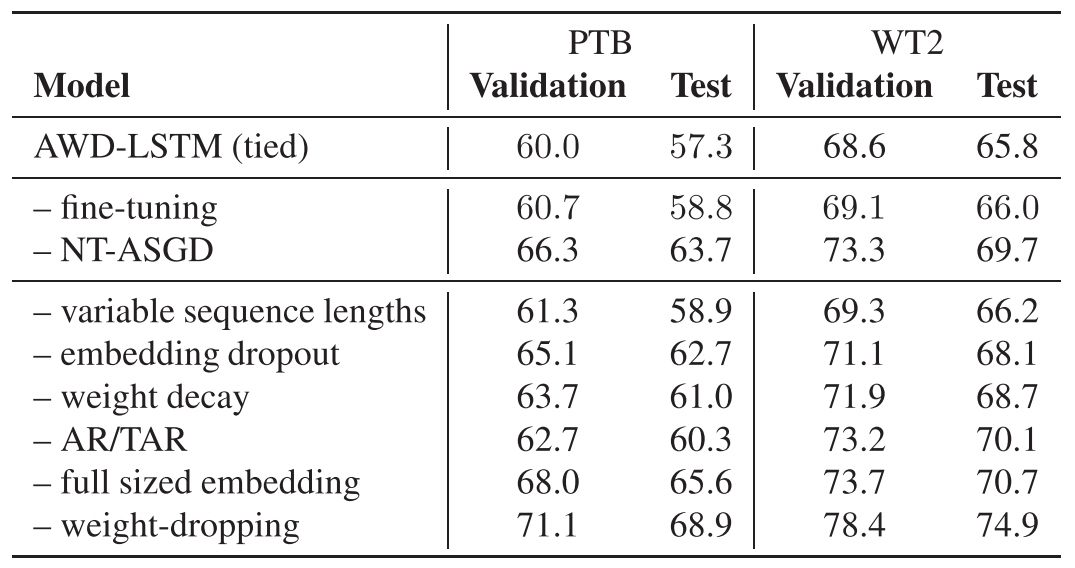
\includegraphics[width=0.9\textwidth]{figures/awdres2.png}
	\end{figure}
\end{itemize}
\end{frame}